\section{Programmorganisationsplan}
\label{sec:programmorganisationsplan}
Im folgenden Abschnitt wird eine Gesamt"ubersicht "uber das Zusammenspiel s"amtlicher Klassen gegeben. Das dazu verwendete UML-Diagram (siehe Abbildung \ref{fig:umlGesamtVereinfacht}, S. \pageref{fig:umlGesamtVereinfacht}) ist leider relativ gro"s geworden. Falls Sie eine vergr"o"serte Version in ihrem Bildbetrachter sehen m"ochten, folgen Sie bitte dem Link in der Lesezeichen- bzw. Anlagen"ubersicht Ihres Pdf-Readers
\footnote{\url{https://www.acrobat-tutorials.de/2013/03/26/dateianlagen-und-seitenanlagen-in-pdf-dokumenten/}}
. Ansonsten liegt das Bild diesem Projekt auch bei (Name \emph{PP18Vereinfacht.png}). 

\embedfilesetup{mimetype=image/png}
\embedfile{programmierhandbuch/Programmorganisationsplan/pics/PP18Vereinfacht.png}

\begin{figure}
	\centering
	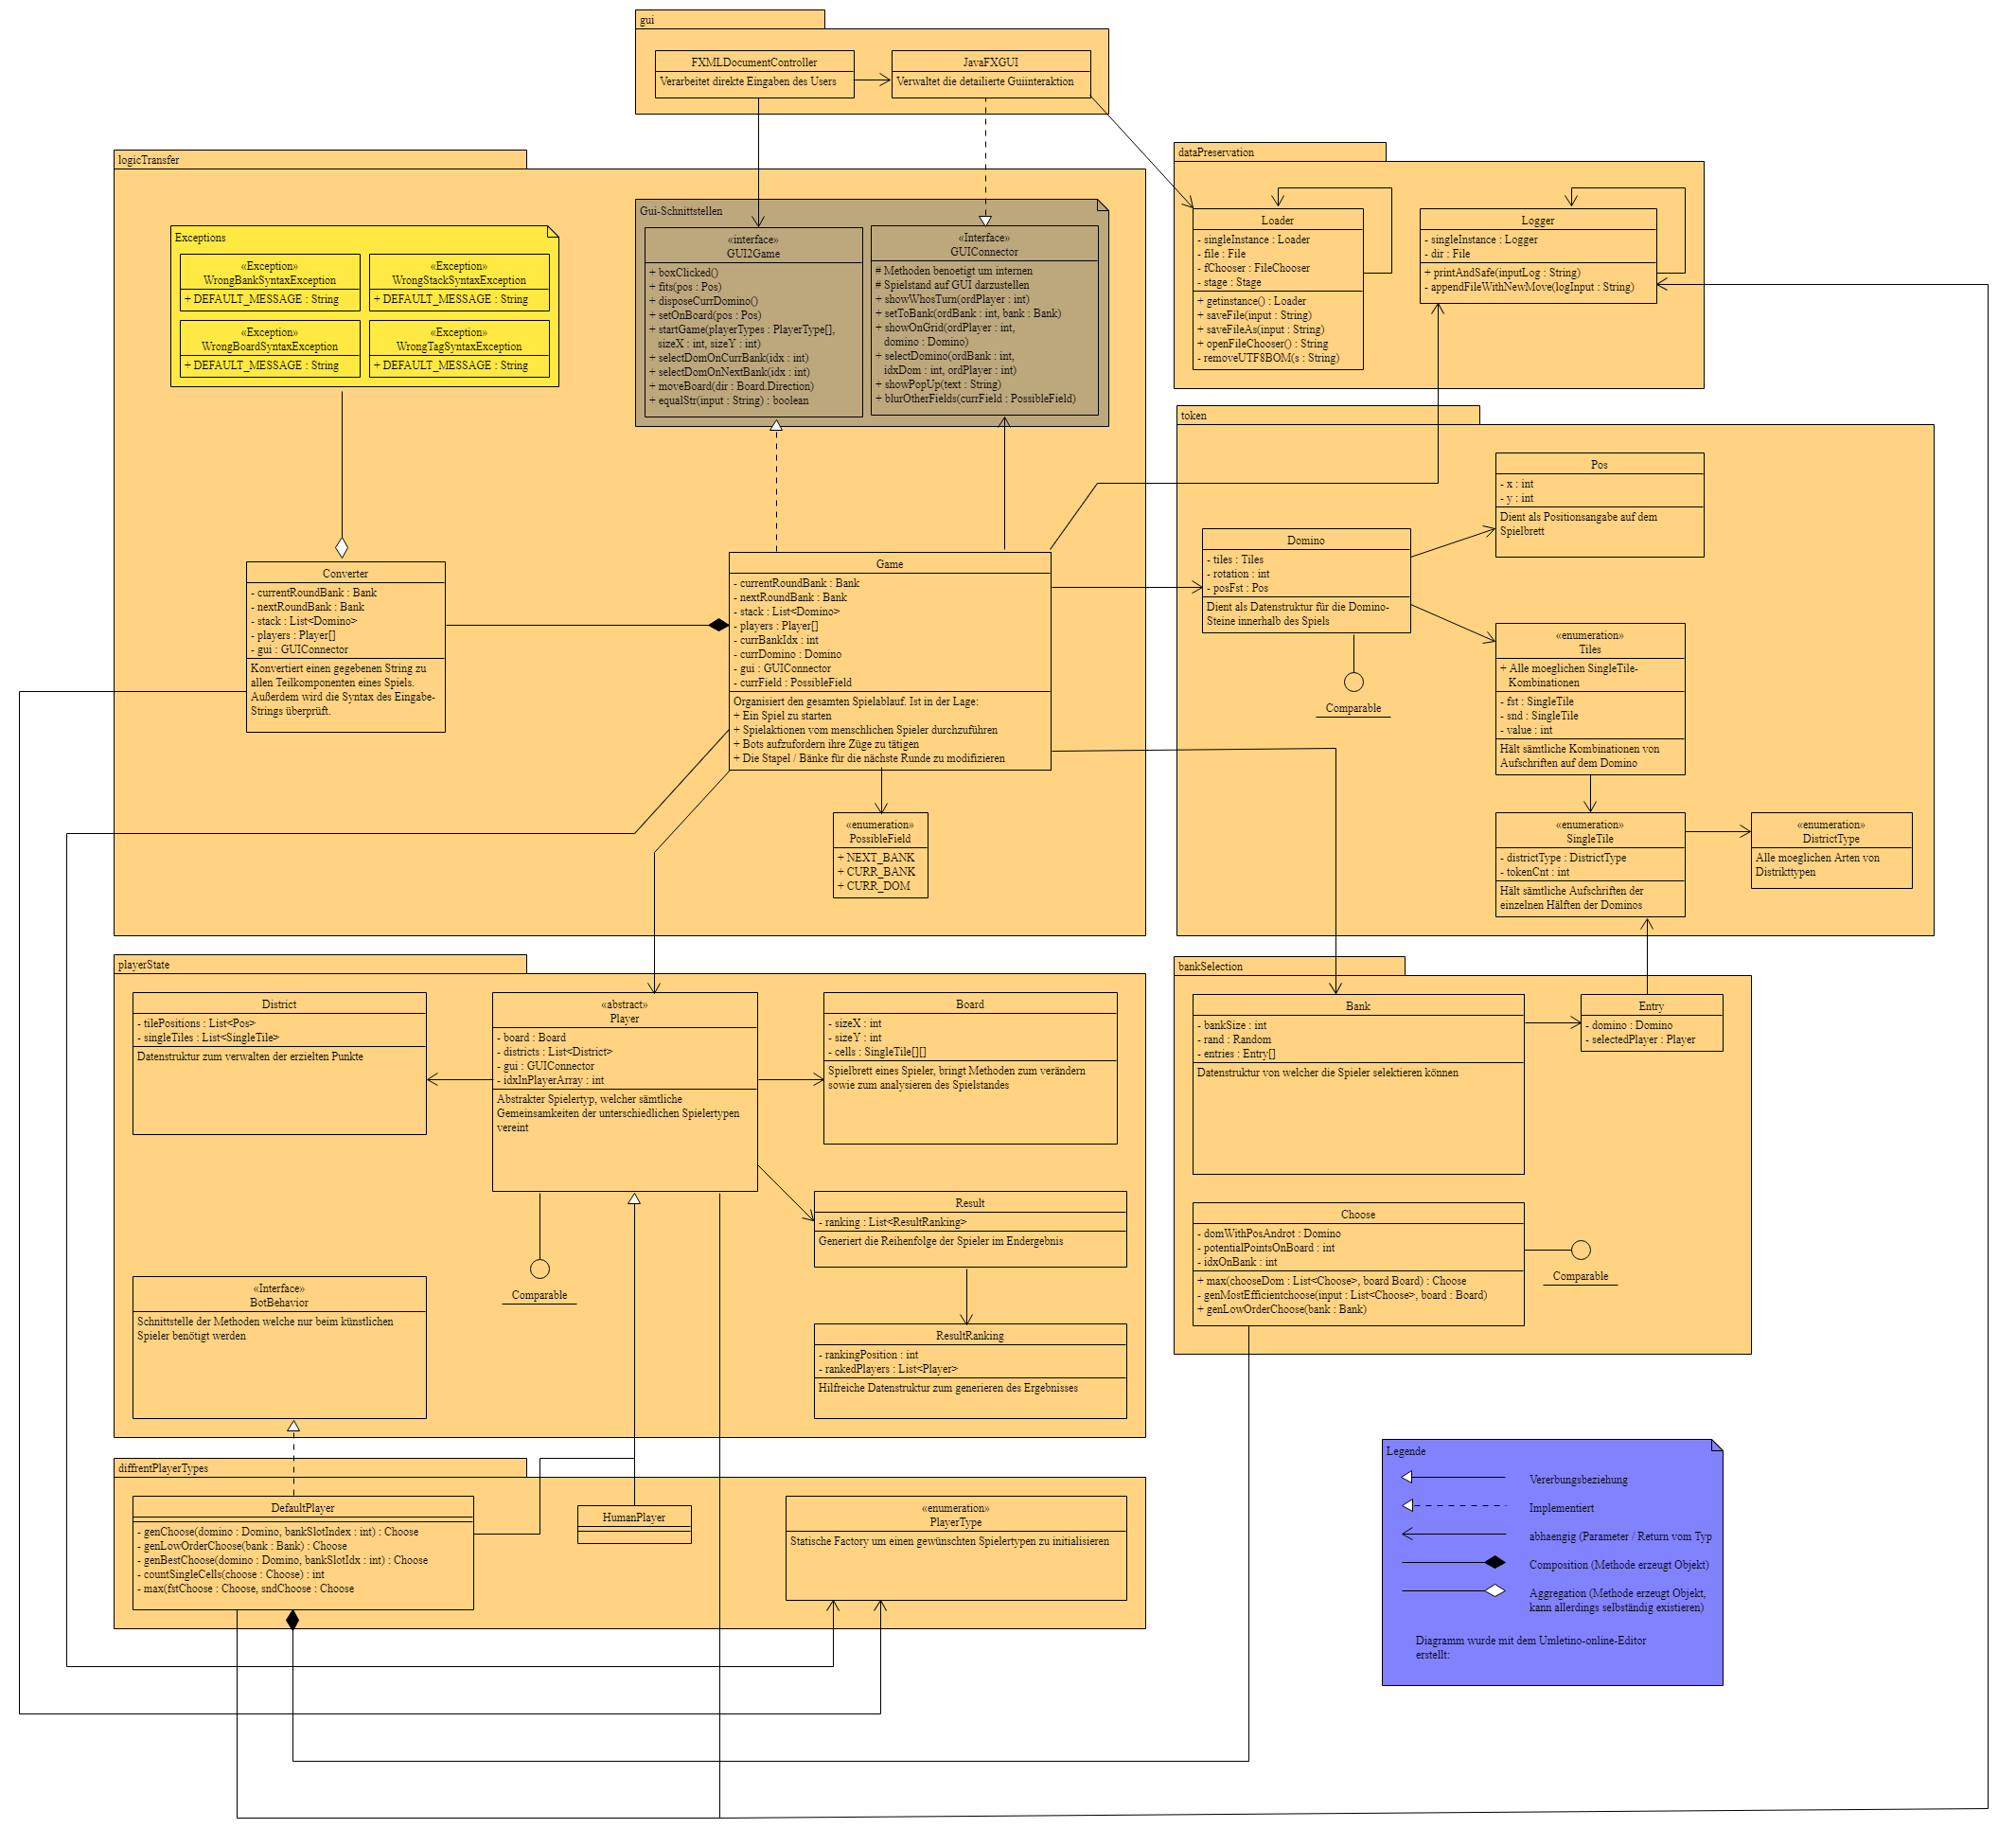
\includegraphics[width=\linewidth]{pics/PP18Vereinfacht}
	\caption{Vereinfachte UML-Darstellung des gesamten Projekts}
	\label{fig:umlGesamtVereinfacht}
\end{figure}

\paragraph{Start einer herk"ommlichen Runde}
Die Klasse, welche die gesammte Anwendung startet, wurde im UML-Diagramm nicht eingezeichnet, da sie nichts anderes tut, als das entsprechende FXML-Dokument zu laden und ein neues Spiel zu starten. Mit dem Laden des FXML-Dokuments wird allerdings auch der dazugeh"orende Controller mit einer initialize-Methode geladen. Diese instantiiert ein JavaFX-Objekt sowie das Spiel selbst. Im Spiel werden alle Teilkomponenten einzeln initialisiert. Es werden demnach alle Spieler, die Gui-Schnittstelle, die B"anke, der Beutel, der aktuelle Bankindex und das gerade betrachtete Feld gesetzt, wobei f"ur dynamische Datenstrukturen hier lediglich ein Typ festgesetzt wird. Die Spieler nehmen hierbei eine besondere Funktion ein, denn sie verwalten intern ihre eigenen Spielfelder, Punkte und Gui-Aktionen. Die Schnittstelle mit dem Spiel soll so minimal wie m"oglich gehalten werden, damit der Spieler m"oglichst autonom handeln kann, um die Erweiterung in einem sp"ateren Entwicklungsstadium mit anderen Spielertypen zu erm"oglichen. Im Konstruktor selbst werden die Spieler allerdings noch nicht instantiiert. Dies geschieht erst in der startGame-Methode. "Ahnlich wie bei den anderen dynamischen Datenstrukturen werden hier die eigentlichen Werte gesetzt. Dazu wird die Hilfsmethode \emph{createNewPlayers} aufgerufen. Diese bekommt einen Array an Spielertypen als \glqq Blaupause\grqq {} f"ur die zu erstellenden Spieler. In der Schleife wird die statische Factory-Methode aufgerufen, welche in der Lage ist, einen gegebenen Spielertypen zu interpretieren und in eine Spielerinstanz umzuwandeln. Der Stack wird nach dem Initialisieren der Spieler ebenfalls gef"ullt. Wieso dieser Aufwand betrieben wurde, wird im Abschnitt \ref{par:alternativeSpielerinitialisierung}, auf Seite \pageref{par:alternativeSpielerinitialisierung} - \nameref{par:alternativeSpielerinitialisierung} beschrieben. 

\paragraph{Selektieren}
Um einen Domino zu selektieren, ben"otigt es eine Spielerreferenz und den Index des Dominos, welcher selektiert werden soll. Die B"anke bestehen aus Entry-Objekten. Ein Entry-Objekt h"alt einen Domino sowie eine Spielerrefernz. 
Auf der Bank ist es m"oglich, einen bisher noch nicht selektierten Eintrag (gekennzeichnet durch einen Null-Pointer an der Stelle der Spielerreferenz des Entry-Objektes) mit der eigenen Spielerreferenz zu "uberschreiben und somit zu selektieren. Wie bereits erw"ahnt, k"onnen die Bots ihre Z"uge selbstst"andig ausf"uhren, wenn sie vom Spiel dazu aufgefordert und mit den entsprechenden Daten versorgt werden. Dabei bedienen Sie sich noch einer Hilfsstruktur (der \emph{Choose}-Klasse) um die Dominos zu untersuchen. Da der menschliche Spieler zu gro"sen Teilen von der Eingabe des Benutzers auf der Gui abh"angt, befinden sich s"amtliche Funktionalit"aten dieses Spielertyps in der Game-Klasse selbst. 

\paragraph{Ablegen}
Mit dem Ablegen eines Steins auf dem Spielfeld muss nicht nur das spielereigene Board erweitert werden, sondern auch die Liste der Distrikte. Dies geschieht bei beiden Spielertypen aber bereits im abstrakten Supertyp Player und muss nicht gesondert behandelt werden. 

\paragraph{Berechnung des Ergebnisses}
Um das Ergebnis zu berechnen wird eine Instanz des Result-Objektes instantiiert. Diese erstellt selbstst"andig eine Liste mit dem Datenobjekt \emph{ResultRanking}. Diese Art des Rankings erlaubt es mehreren Spielern denselben Platz zuzuweisen und bringt selbst noch einige hilfreiche Methoden, um die gesamte Rechnung sowie Darstellung zu vereinfachen. 

\paragraph{Logging}
Die Logger-Klasse nimmt eine Sonderrolle ein, da sie nichts anderes tut als eine Nachricht abzuspeichern. Dies wird immer genutzt, wenn es darum geht, ein Zwischenergebnis festzuhalten. Daher wird sie in relativ vielen Klassen verwendet. 

\begin{lstlisting}[style=CodeHighlighting,caption=Game - startGame,label=game_startGame]
@Override
public void startGame(PlayerType[] playerTypes, int sizeX, int sizeY) {
    // instanciate players with given playertypes
    this.players = createNewPlayers(playerTypes, sizeX, sizeY);

    for (int i = 0; i < this.players.length; i++) {
        this.gui.updatePlayer(this.players[i]);
    }

    // fill stack
    this.stack = Domino.fill(this.stack);

    // fill current bank
    this.stack = this.currentRoundBank.randomlyDrawFromStack(this.stack);
    this.gui.setToBank(CURRENT_BANK_IDX, this.currentRoundBank);

    this.currBankIdx = 0;
    this.gui.showWhosTurn(HUMAN_PLAYER_IDX);

    Logger.getInstance().printAndSafe(Logger.GAME_SEPARATOR + "\nStarted new game\n");
}

private Player[] createNewPlayers(PlayerType[] playerTypes, int sizeX, int sizeY) {
    Player[] output = new Player[playerTypes.length];
    for (int i = 0; i < playerTypes.length; i++) {
        output[i] = PlayerType.getPlayerInstanceWithGivenType(playerTypes[i], i, 
        		this.gui, sizeX, sizeY);
    }
    return output;
}
\end{lstlisting}